\subsection{Loss functions}
The problem of decoy quality assessment is essentially a ranking
problem: we have to arrange decoys according to their similarity to
the corresponding native structure, as quantified by the GDT\_TS score
\cite{zemla2001casp4}, for instance. Such a ranking approach to the
problem of model quality assessment has recently been used by the
MQAPRank method \cite{jing2016sorting}, which, however, relies on a
support vector machine architecture and uses high-level features as
input.
%%% GL: Ranking is a very common task, so I don't see the usefulness
%%% of citing gong2013deep.
%%% GL: Every paper I see seems to be calling it ``GDT_TS'', not
%%% ``GDT-TS'' (underscore, not dash).

In the present work, we define the loss function in terms the margin
ranking loss for each pair of decoys. Let a decoy representation be
denoted as $x_i$ and the output of the network for this decoy as
$f(x_i)$. Let $y_{ij}$ be the ordering coefficient of the two decoys:
$$
y_{ij} = \begin{cases}
               1& \text{if }\text{GDT\_TS}_i \leq \text{GDT\_TS}_j \\
               -1& \text{if }\text{GDT\_TS}_i > \text{GDT\_TS}_j \\
            \end{cases}
$$
%
Here, $\text{GDT\_TS}_i$ is the global distance test total score of
the $i$-th decoy. We use the following expression for the pairwise
ranking scoring function:
$$
L_{ij} = w_{ij} \cdot \max \left[ 0, 1 - y_{ij} \left( f \left( x_i \right) - f \left( x_j \right) \right) \right]]
$$
%
The term $w_{ij}$ represents an example weight:
%
$$
w_{ij} = \begin{cases}
               1& \text{if } \left| \text{GDT\_TS}_i - \text{GDT\_TS}_j \right| > T \\
               0& \text{otherwise} \\ 
            \end{cases}
$$
%
where $T$ is a threshold constant set to 0.1~{\AA}. This has the
effect of avoiding to train the model on pairs of decoys that are too
similar.

During the training procedure we load $N_\text{B}$ decoy structures of
a given target into memory (a ``minibatch'') and compute the output of the
network and the average loss:
$$ L = \frac{1}{N^{2}_\text{B}} \sum_{i=1,j=1, i \neq j}^{N_\text{B}} L_{ij} $$
Afterwards, we compute the gradient of the average loss with respect
to the network parameters and update them using the Adam algorithm
\cite{???}.
%%% GL: What value of N_B are we using??? This should be answered here...


\subsection{Evaluation criteria}
\tchanged{
We evaluated our algorithm using the correlation coefficients and loss criterions. The correlation coefficents 
were computed between the score of our model and GDT\_TS metric for all the decoys of each target protein in a test set and then averaged.
}
The loss criterion is the deviation of the GDT\_TS of the best decoys for a protein from the GDT\_TS score of the decoy with the lowest score:
$$ 
Loss = | max_i( \text{GDT\_TS}_i ) - \text{GDT\_TS}_{argmin_i(f(x_i))} |
$$ 

\subsection{Optimization and dataset sampling}
The optimization procedure of deep convolutional networks usually is stochastic: the function value and gradient 
is estimated on a small subset (batch) of all the training 
examples. We used the batch of size 10 due to the memory limitations. Afterward the parameters of the model are 
changed in the direction of the estimated gradient.
The parameter update step was performed using the Adam algorithm \cite{kingma2014adam}. 

The dataset was sampled in the following way: first we chose a random protein from the dataset, then we sample decoys of this protein. 
The procedure is repeated for all the 
proteins in a dataset. One pass through all the proteins in a dataset is called epoch. 
The decoys are sampled in a homogeneous way: we divide all the decoys into $M$ clusters by the value of GDT\_TS score. 
Precisely, the decoy $i$ belongs to the cluster  
number $ \left[ \frac{\max(\text{GDT\_TS}) - \text{GDT\_TS}_i}{\max(\text{GDT\_TS}) - \min(\text{GDT\_TS})} \right] + 1$, 
where $\max(\text{GDT\_TS})$ and $\min(\text{GDT\_TS})$ are computed for all the decoys of 
the chosen protein. If there are empty clusters, then we take secon decoys from each non-empty and so on until we filled the batch. 
At the end of each epoch we randomly shuffle the order of protein and the order of decoys in each cluster. 

Each decoy from the selected batch is randomly rotated and translated. The rotations are sampled uniformly \cite{shoemake1992uniform}. 
The translation are chosen in such a way, that the bounding box of the translated protein lies within the box of the size 120x120x120\AA. 

To select the final model we randomly divided the training set into training and validation subsets. The validation subset consists of 
35 targets and their decoys. This subset was not sampled during the training. 
Figure \ref{Fig:TrainingLoss} shows the Kendal tau, Pearsor R coefficients and the loss on the vaidation subset. 
The final model was chosen according to the minimum loss (epoch 40).
\begin{figure}[H]
    \centering
    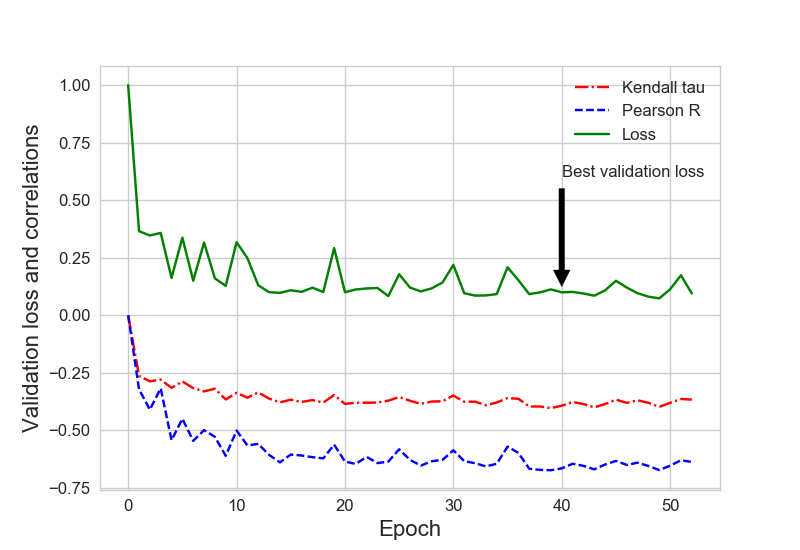
\includegraphics[width=\linewidth]{Fig/kendall_validation.eps}
    \caption{The loss, Kendal tau and Pearson R coefficients evaluated on the validation subset during the training procedure. 
    The epoch denotes that all the targets in the training subset were sampled. The arrow shows the minimum validation loss 
    among epochs divisible by 10 (we saved our model each 10 epoch).}
    \label{Fig:TrainingLoss}
\end{figure}

The table \ref{Tbl:TrainingResults} summarizes the performance metrics on the training and validation sets for the model at epoch 40.

\begin{table}[H]
\begin{center}
\begin{tabular}{ c | c | c | c | c }
    Data subset & Loss & Pearson & Spearmann & Kendall \\
    \hline
    Training set     &0.146 &0.71 &0.61 &0.45 \\
    Validation set   &0.135 &0.71 &0.59 &0.44 \\ \hline

\end{tabular}
  \caption {Results of the model from epoch 40 on the training and validation subsets.}
    \label{Tbl:TrainingResults}
\end{center}
\end{table}
